% Load preamble
\documentclass[../main.tex]{subfiles}

\begin{document}
    \subsection{Príklad prvý}
	    Majme systém, ktorý je určený stavovým opisom \cref{eqn:svlvvPr1SyavovyOpis}. Bloková schéma systému je na \cref{fig:svlvvPr1BlockSchemaSystemu}.
	\begin{equation}
		\begin{gathered}
		\dot{x_1}  =u + \sin(x_1) x_2 \\
		\dot{x_2} = 2x_1 + sin(x_1) \\
		y = x_2
		\end{gathered}
		\label{eqn:svlvvPr1SyavovyOpis}
	\end{equation}
	\begin{figure}[h!]
		\centering
		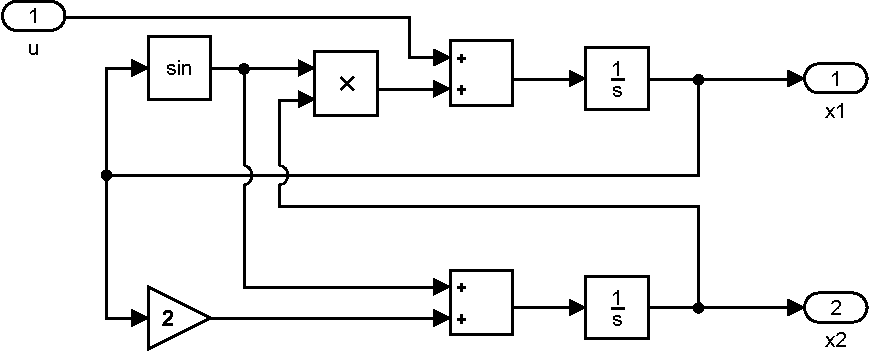
\includegraphics[width=0.8\linewidth]{svlvvPr1/svlvvPr1Sys-crop}
		\caption{Bloková schéma systému z \cref{eqn:svlvvPr1SyavovyOpis}}
		\label{fig:svlvvPr1BlockSchemaSystemu}
	\end{figure}
	
	Predpokladajme, že chceme tento systém riadiť tak, aby výstup dosiahol žiadanú hodnotu $r$ a aplikujme nelineárne riadenie navrhnuté metódou vstupno výstupnej spätnoväzobnej linearizácie. Metódu vysvetlíme rovno počas návrhu. 
	
    \subsubsection{Prvý krok - derivácia rovnice výstupu}
    Prvým krokom metódy je derivácia vzťahu pre výstup systému $y$. Derivujeme toľkokrát koľkokrát je potrebné, nato aby sa vstup systému $u$ objavil v rovnici.
	\begin{equation*}
	\begin{aligned}
		y &= x_2 \\ 
		\implies \dot{y}  &= \dot{x_2} =  2x_1 + sin(x_1) \\
		\implies \ddot{y} &= \ddot{x_2} \\
						  &= 2 + cos(x_1)\dot{x_1} \\
						  &= 2 + \cos(x_1)(u + \sin(x_1) x_2)
		\end{aligned}
		\label{eqn:}
	\end{equation*}
    vo výsledku dostaneme vzťah \cref{eqn:svlvvpr1-derivv}.
    \begin{equation}
        \begin{aligned}
            \ddot{y} = 2 + \cos(x_1)(u + \sin(x_1) x_2) \\
        \end{aligned}
        \label{eqn:svlvvpr1-derivv}
    \end{equation} 

    \subsubsection{Druhý krok - voľba zákona linearizácie}
	Teraz si všimnime, že ak zvolíme vstup $u$ do systému, tak ako je \cref{eqn:svlvvPr1ZakonLinearizacie} 
	\begin{equation}
	    u = -\sin(x_1) x_2  +  \frac{v}{2 + \cos x_1}
	    \label{eqn:svlvvPr1ZakonLinearizacie}
	\end{equation}
po dosadení do \cref{eqn:svlvvpr1-derivv} dostaneme:% \cref{eqn:svlvvPr1-dosadenie}.
	\begin{equation*}
	\begin{aligned}
	 	\ddot{y} &= 2 + \cos(x_1)(u + \sin(x_1) x_2) \\
	 		     &= 2 + \cos(x_1)(-\sin(x_1) x_2  +  \frac{v}{2 + \cos x_1} + \sin(x_1) x_2)  \\ 
	 		     &= 2 + \cos(x_1)(\frac{v}{2 + \cos x_1})  \\ 
	 		     &= v  \\ 
 	\end{aligned}
	%\label{eqn:svlvvPr1-dosadenie}
	\end{equation*}
    Dostávame tak vzťah medzi výstupom systému $y$ a vstupom do zákona linearizácie $v$ v \cref{eqn:svlvvpr1-yvvztah}.
    \begin{equation}
        \begin{aligned}
            \ddot{y} = v
        \end{aligned}
        \label{eqn:svlvvpr1-yvvztah}
    \end{equation} 
     Voľba takéhoto zákona, nazvime ho zákonom linearizácie, pre vstup $u$ do systému, je druhým krokom metódy.

    \subsubsection{Tretí krok - návrh lineárneho zákona riadenia}
    Ako posledný krok, musíme zvoliť tvar $v$, tak aby sme dosiahli požadovanú dynamiku systému.
    
    Zvolme si $v$ podľa \cref{eqn:svlvvPr1ZakonRiadenia}.
	\begin{equation}
	\begin{aligned}
	 v &= \ddot{r}  +k_1 \dot{e} + k_0 e \\
	   &= -k_1 \dot{y} + k_0 e \text{ keďže $r$ je konšt., tak jeho derivácie sú 0}\\
	   \end{aligned}
	\label{eqn:svlvvPr1ZakonRiadenia}
	\end{equation}
    potom dosadením \cref{eqn:svlvvPr1ZakonRiadenia} do \cref{eqn:svlvvpr1-yvvztah} dostaneme 
	\begin{equation*}
	\begin{aligned}
	 \ddot{y} &= \ddot{r}  +k_1 \dot{e} + k_0 e \\
	 0 &= \ddot{e}  + k_1 \dot{e} + k_0 e \\
	\end{aligned}
	\end{equation*}
    pre takúto voľbu $v$ bude teda pre systém platiť \cref{eqn:svlvvpr1-dynodch}.
    \begin{equation}
        \begin{aligned}
	        0 &= \ddot{e}  + k_1 \dot{e} + k_0 e \\
        \end{aligned}
        \label{eqn:svlvvpr1-dynodch}
    \end{equation} 
    kde $k_1$ a $k_0$ sú voliteľné parametre. 

    Parametre $k_1$ a $k_0$ vieme tiež navrhnúť podľa potreby. Ak si prepíšeme \cref{eqn:svlvvpr1-dynodch} na \cref{eqn:svlvvpr1-dynodch2}.
    \begin{equation}
        \begin{aligned}
	        r_e &= \ddot{e}  + k_1 \dot{e} + k_0 e \\
        \end{aligned}
        \label{eqn:svlvvpr1-dynodch2}
    \end{equation} 
    kde $r_e$ bude žiadaná hodnota odchýlky (ktorá je 0), tak vieme vyjadriť prenos $\frac{e}{r_e}$:
    \begin{equation*}
        \begin{aligned}
	        r_e &= \ddot{e}  + k_1 \dot{e} + k_0 e \\
            R_e &= Es^2  + k_1Es  + k_0E  \\
            R_e &= E(s^2  + k_1s  + k_0)  \\
            \frac{E}{R_e} &= \frac{1}{s^2  + k_1s  + k_0} \\
        \end{aligned}
        \label{eqn:}
    \end{equation*} 
    charakteristický polynóm teda bude \cref{eqn:svlvvPr1-odchchp}.
    \begin{equation}
        \begin{aligned}
            s^2  + k_1s  + k_0 = 0
        \end{aligned}
        \label{eqn:svlvvPr1-odchchp}
    \end{equation} 
    zvolíme žiadanú polohu pólov $p_1, p_2$ potom žiadaný charakteristický polynóm bude \cref{eqn:svlvvPr1-ziadchp}.
    \begin{equation}
        \begin{aligned}
            (s - p_1)(s-p_2) = s^2 - (p_1 + p_2)s + p_1p_2
        \end{aligned}
        \label{eqn:svlvvPr1-ziadchp}
    \end{equation} 
    porovnaním \cref{eqn:svlvvPr1-odchchp} a \cref{eqn:svlvvPr1-ziadchp} dostaneme sústavu rovníc \cref{eqn:svlvvPr1-odhcpp}.
    \begin{equation}
        \begin{aligned}
            p_1p_2 &= k_0 \\
            -(p_1 + p_2) &= k_1 \\
        \end{aligned}
        \label{eqn:svlvvPr1-odhcpp}
    \end{equation} 
    cez ktoré vieme vypočítať $k_1$ a $k_0$ pre ľubovoľné žiadané póly.

    Zvolme si $p_1 = -1$ a $p_2 = -1$ potom z \cref{eqn:svlvvPr1-odhcpp} dostaneme $k_1=2$ a $k_2 = 1$

	Máme tak navrhnutý regulátor. Výsledok overíme simuláciou, pre niekoľko žiadaných úrovní výstupu. Priebehy zo simulácie sú na \cref{fig:svlvvPr1Vysledok}.
	\begin{figure}[h!]
		\centering
		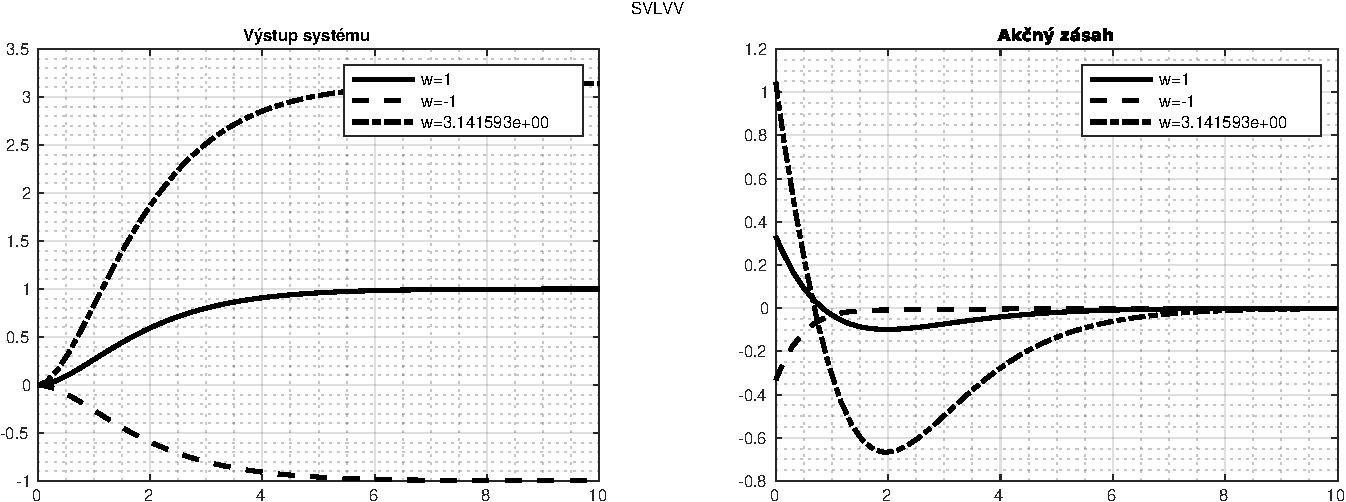
\includegraphics[width=\linewidth]{svlvvPr1/svlvvPr1Vysledok-crop}
		\caption{Regulácia výstupu na konštantnú hodnotu nelin. regulátorom navrhnutým pomocou metódy spätnoväzbovej linearizácie vstupno-výstupnej \cref{eqn:svlvvPr1SyavovyOpis}}
		\label{fig:svlvvPr1Vysledok}
	\end{figure}

    \subsubsection{Zhrnutie krokov metódy}
    Kroky návrhu sumarizujeme v 3 bodoch:
    \begin{enumerate}
        \item Derivácia rovnice výstupu, až kým sa v rovnici neobjaví vstupná premenná
        \item Voľba zákona linearizácie (napríklad odčítanie nelineárnych zložiek)
        \item Návrh zákona riadenia (regulátora) pre linearizovaný systém
    \end{enumerate}

    \subsubsection{Rovnovážny stav systému}
    Bod $x_1 = x_2 = 0$ je rovnovážnym bodom tohto systému, čo si môžeme overiť dosadením:
	\begin{equation*}
	    \begin{aligned}
            \dot{x_1}|_{(x_1 = x_2 = 0)} &= \sin(0) 0 = 0 \\
            \dot{x_2}|_{(x_1 = x_2 = 0)}  &= 0 + sin(0) = 0 \\
	    \end{aligned}
	    \label{eqn:svlvvPr1OverenieRB}
	\end{equation*}

	všimnime si, že v tomto bode sú derivácie stavových premenných v čase nulové, čo je charakteristické pre rovnovážne body.
    \subsubsection{Porovnanie s PID}
	Pre porovnanie skúsme navrhnúť ešte PID regulátor pre systém linearizovaný v rovnovážnom bode $x_1 = x_2 = 0$. Po linearizovaný bude mať systém tvar \cref{eqn:svlvvPr1LinearizovanySystem}. 
	\begin{equation}
	\begin{gathered}
	\Delta \dot{x_1}  = \Delta u \\
	\Delta \dot{x_2} = 3\Delta x_1 \\
	\Delta y = \Delta  x_2
	\end{gathered}
	\label{eqn:svlvvPr1LinearizovanySystem}
	\end{equation}

	Vyjadrime si prenosovú funkciu systému, pre jednoduchší návrh parametrov regulátora. Vyjadrenie prebieha v \cref{eqn:svlvvPr1VyjadreniePrenosuLinSys}. V tomto momente ešte potrebujeme zapojiť pred systém regulátor a vyjadriť prenos uzavretého regulačného obvodu.
	\begin{equation}
	\begin{aligned}
		\Delta  y &= \Delta x_2 = \frac{1}{s}  3 \Delta x_1 = \frac{1}{s^2}  3 \Delta u \\
		\implies \frac{\Delta y}{\Delta u } &= \frac{3}{s^2} \\
	\end{aligned}
	\label{eqn:svlvvPr1VyjadreniePrenosuLinSys}
	\end{equation}
	Zapojme na vstup systému PID regulátor, ako je na \cref{fig:svlvvPr1ZapojeinePIDNaLinSys}. Ktorý má prenos \cref{eqn:svlvvPr1PIDPrenos}, kde $P, D, I$ sú parametre regulátora. Pre zjednodušenie ešte prenosy systému a regulátora roznásobme, dostaneme tak prenos otvoreného obvodu $G_{ORO}$ daný \cref{eqn:svlvvPr1PIDPrenosORO}. 
	\begin{figure}[h!]
		\centering
		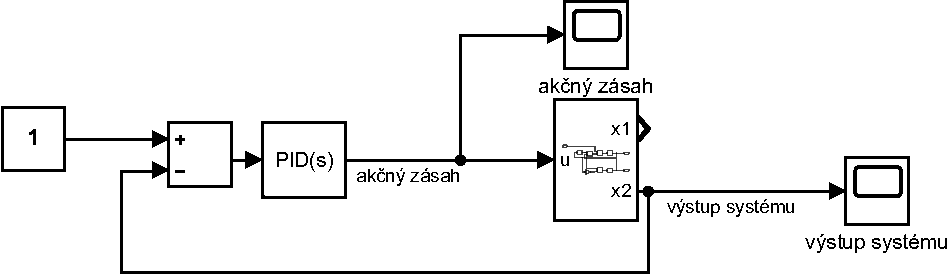
\includegraphics[width=0.8\linewidth]{svlvvPr1/svlvvPr1ZapojeniePID-crop}
		\caption{Zapojenie PID regulátora}
		\label{fig:svlvvPr1ZapojeinePIDNaLinSys}
	\end{figure}
	\begin{equation}
		\begin{aligned}
			\frac{U(s)}{E(s)} = P + Ds + \frac{I}{s} \\
		\end{aligned}
		\label{eqn:svlvvPr1PIDPrenos}
	\end{equation}
	\begin{equation}
	\begin{aligned}
	G_{ORO} = 3\frac{Ps + Ds^2 + I}{s^3} \\
	\end{aligned}
	\label{eqn:svlvvPr1PIDPrenosORO}
	\end{equation}
	Následne vyjadrime prenos uzavretého regulačného obvodu $G_{URO}$ podľa známeho pravidla zápornej spätnej väzby \cref{eqn:svlvvPr1PravidloZapornejSpantejVazby}. Dostaneme tak prenos \cref{eqn:svlvvPr1PrenosURO}.
	\begin{equation}
			\begin{aligned}
			G_{URO} = \frac{G_{ORO}}{1 + G_{ORO}}
			\end{aligned}
			\label{eqn:svlvvPr1PravidloZapornejSpantejVazby}
	\end{equation}
	\begin{equation}
		\begin{aligned}
		G_{URO} &= \frac{3\frac{Ps + Ds^2 + I}{s^3}}{1 + 3\frac{Ps + Ds^2 + I}{s^3}}  \\
		 		&= \frac{3(Ps + Ds^2 + I)}{s^3 + 3Ps + 3Ds^2 + 3I}
		\end{aligned}
		\label{eqn:svlvvPr1PrenosURO}
	\end{equation}
	Využime teraz metódu pole-placement na návrh parametrov regulátora, umiestnime póly na týchto pozíciách komplexnej roviny $p_1 = -1, p_2 = -1, p_3 = -1$. Teda nech sú póly reálne a záporné, čo zabezpečí stabilitu lineárneho systému, keďže na kvalitu riadenia zatiaľ nekladieme dôraz.

	Polynóm, ktorý bude mať zvolené korene, získame roznásobením polynómov prvého stupňa, ktorých korene sú zvolené póly, teda roznásobením \cref{eqn:svlvvPr1VznikZiadanehoPolynomu}. 
		\begin{equation}
	\begin{aligned}
	P(s) &= (s - p_1)(s - p_2)(s - p_3) \\
		 &= (s + 1)(s + 1)(s + 1) \\
		 &= s^3 + 3s^2 + 3s + 1\\
	\end{aligned}
	\label{eqn:svlvvPr1VznikZiadanehoPolynomu}
	\end{equation}
	Tento želaný polynóm porovnáme s charakteristickým polynómom uzavretého regulačného obvodu, teda \cref{eqn:svlvvPr1Porovnanie}, dostaneme tak rovnice \cref{eqn:svlvvPr1RovniceParametrovPID} z ktorých vypočítame parametre regulátora.
	\begin{equation}
	\begin{aligned}
		s^3 + 3s^2 + 3s + 1= s^3 + 3Ps + 3Ds^2 + 3I\\
	\end{aligned}
	\label{eqn:svlvvPr1Porovnanie}
	\end{equation}
	\begin{equation}
	\begin{aligned}
		\begin{matrix}
		3P &= 3 \\
		3D &= 3 \\ 
		3I &= 1 \\
		\end{matrix}
		\implies 
		\begin{matrix}
		P &= 1 \\
		D &= 1 \\ 
		I &= \frac{1}{3}  \\
		\end{matrix}
	\end{aligned}
	\label{eqn:svlvvPr1RovniceParametrovPID}
	\end{equation}

    Najprv aplikujme tento regulátor na linearizovaný systém, aby sme si overili návrh. Výsledok zo simulácie je na \cref{fig:svlvvPr1VysledokPIDLin}.
    \begin{figure}[h!]
        \centering 
        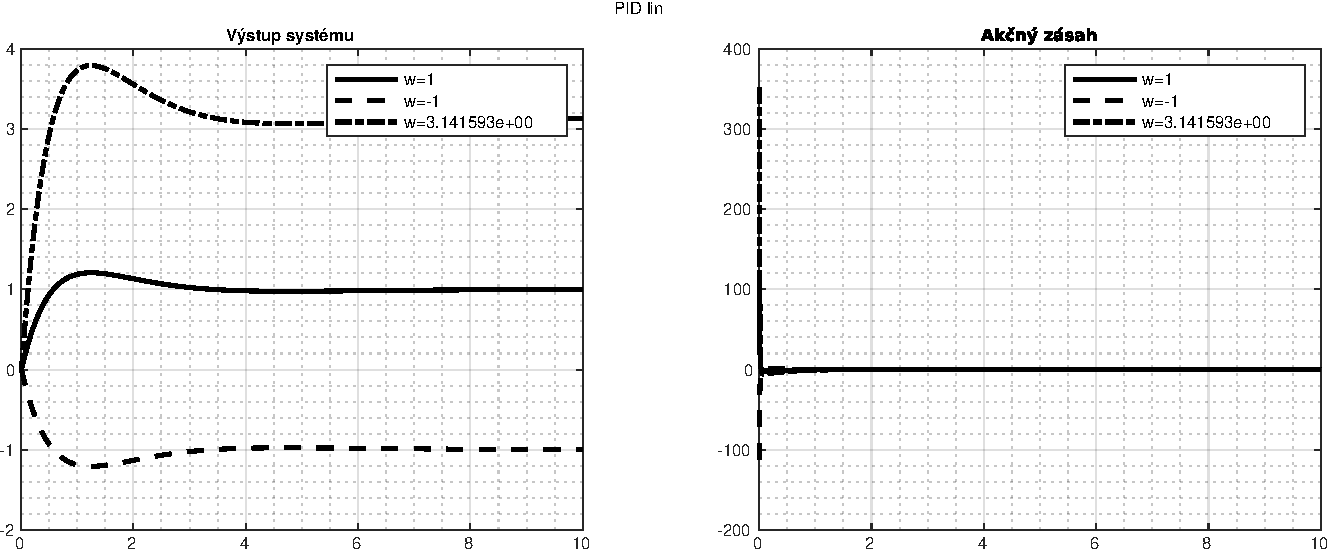
\includegraphics[width=\linewidth]{svlvvPr1/svlvvPr1PIDVysledokLin-crop}
        \caption{PID regulátor na linearizácii systému v pracovnom bode}
        \label{fig:svlvvPr1VysledokPIDLin}
    \end{figure} 

	Aplikujme teraz PID regulátor aj na nelineárny systém, ktorý chceme riadiť. Výsledok zo simulácie je na \cref{fig:svlvPr1VysledokPID}.
		\begin{figure}[h!]
			\centering
		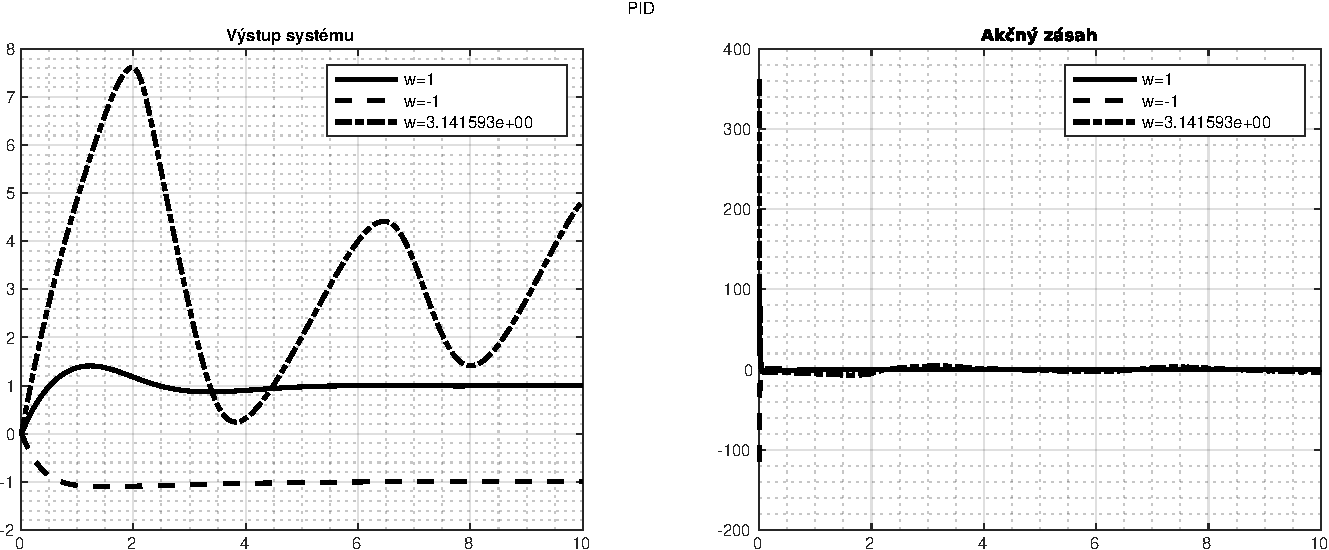
\includegraphics[width=\linewidth]{svlvvPr1/svlvvPr1PIDVysledok-crop}
		\caption{PID regulátor na nelineárnom systéme}
		\label{fig:svlvPr1VysledokPID}
	\end{figure}

    Vidíme ako PID regulátor zvláda riadenie pre istú oblasť žiadaných hodnôt, kde sa linearizácia nelineárneho systému nelíši do veľkej miery od pôvodného systému.

    Avšak pre väčšie skoky PID regulátor prestáva fungovať ako to vidíme pre skok $w=\pi$.
	Z výsledku môžeme usúdiť, že použiť nelineárne riadenie je v niektorých prípadoch nevyhnutné.
\end{document}
